 \documentclass{ctexart}

\usepackage[english]{babel}
\usepackage[utf8]{inputenc}
\usepackage{hyperref}
\usepackage{amsmath}
\usepackage{amssymb}
\usepackage{tikz}
\usetikzlibrary{positioning}
\usepackage{graphicx}
\usepackage[colorinlistoftodos]{todonotes}

%\usepackage[utf8]{ctex/option}

\title{探索深度学习方法在时间序列分析问题上的可行性--利用神经网络与小波分析进行变点检测}

\author{郭森辉,郑哲诗,李玉桥}

\date{\today}

\begin{document}
\maketitle

\begin{abstract}
在本篇报告中,我们提出利用神经网络对高度非线性数据的良好拟合能力,通过在经过小波分解后的时间序列数据上训练网络,获得了一个置信度相当高的变点判别模型。同时由于神经网络是非参数的(其参数只取决于结构而非其中的参数),该方法有很好的泛化性。而又由于小波的局部性,该方法可用于实时变点检测。
\end{abstract}

\section{介绍}
\label{sec:introduction}

变点检测是时间序列分析中的一个基本问题,也是机器学习中的一个基本问题。传统的方法有CUSUM、double CUSUM等其变种,似然商法,核方法,图方法等,由于时间序列本身的复杂性以及估计方法的缺失,以上方法往往限制于低阶时间序列(二阶及以下),高阶非平稳以及高维情形下的变点分析至今仍然是空白。同时由于分析方式的局限性,传统方法对于序列只能进行离线检测,无法进行实时变点分析。考虑到深度学习方法对高度非线性模型的良好拟合效果,我们提出可以将时间序列数据化以后用于网络的训练从而来产生对特定或者多类型变点的分类/判别器。

\section{背景以及相关工作}
\label{sec:theory}

\subsection{传统变点检测方法}

\subsection{小波分析与时间序列}
我们知道,对于一个时域上的序列我们可以对其进行傅立叶变换从而得到其频域上的信息(能量谱密度),然而使用傅立叶变换之后所有时域上的信息都消失了,此时我们无法对一个时间序列进行局部分析。后来人们引进窗口傅立叶,通过牺牲频域上的精确度来获得时域上的局部信息,然而窗口傅立叶理论并不完备,实际应用效果不好。直到后来人们找到了完备化的窗口傅立叶,也就是我们在本文中用于将时间序列数据化的小波分析,此时我们对时域上的序列的频率/能量分析进入了一个新的时代。\\
小波变换的本质和傅立叶变换类似,也是用挑选的基来表示信号方程。每个小波变换都会有一个mother wavelet,我们称之为母小波,同时还有一个scaling function,即尺度函数,也被称为父小波。在某一尺度下小波变换的基函数是一系列母函数的线性组合,而父函数可以将母函数扩展到分辨率更高的空间。\\
小波展开的通常形式是:
\begin{equation}
  f(t)=\sum_{k=-\infty}^\infty c_k\phi(t-k)+\sum_{k=-\infty}^\infty \sum_{j=0}^\infty d_{j,k}\psi(2^jt-k)
\end{equation}
以本文使用的小波函数:哈尔小波为例,哈尔小波具有以下形式:
\begin{equation}
   \psi(n)=
   \begin{cases}
    \frac{1}{2\sqrt{2}} &1\leq n\leq4\\
    -\frac{1}{2\sqrt{2}} &5\leq n\le8\\
    0 &o.w.
   \end{cases}
\end{equation}
哈尔小波是最简单的小波,同时也是现在使用最多最广泛的小波。总而言之,通过小波分析对于时域序列的局部频率分析能力,我们能够将特定时间点的时间序列数字化,以简单向量的形式呈现,下面是有变点和无变点情形下变点处的能量谱(Figure 1):
\begin{figure}
  \centering
  \includegraphics[width=0.9\textwidth]{coef.jpg}
  \caption{不同变点情形下时间序列的能量谱}
\end{figure}

\subsection{神经网络以及深度学习}
神经网络与深度学习是最近最流行的模型拟合方法,因其强大的对非线性以及高度复杂的模型的拟合能力而被应用在各个地方。其原理(Figure 2)很简单, 通过相对复杂网络结构以及激活函数来构造一个能够产生高度非线性函数的模型,在训练数据上通过梯度下降法来训练模型,从而使其对训练数据的拟合效果更好(这里的效果好是我们自己定义的,在本文中我们使用了交叉熵函数作为损失函数),同时避免过拟合。换句话说,每一个固定的网络结构(不包含结构中参数的具体取值)代表了一个函数类,而网络的训练即是找到我们想要的那个函数(即一套参数)。\\
而深度学习则是加深版的神经网络,由于之前激活函数的限制导致梯度消失,从而无法完成训练,通过新的激活函数以及特别的训练技巧,还有强大的计算能力,我们现在已经能够训练上百层的神经网络,这也意味这函数类将越来越大,越来越复杂,我们能通过神经网络描述的复杂模型的范围也越来越大,这其中就包括时间序列。
\tikzset{%
  every neuron/.style={
    circle,
    draw,
    minimum size=1cm
  },
  neuron missing/.style={
    draw=none,
    scale=4,
    text height=0.333cm,
    execute at begin node=\color{black}$\vdots$
  },
}
\begin{figure}
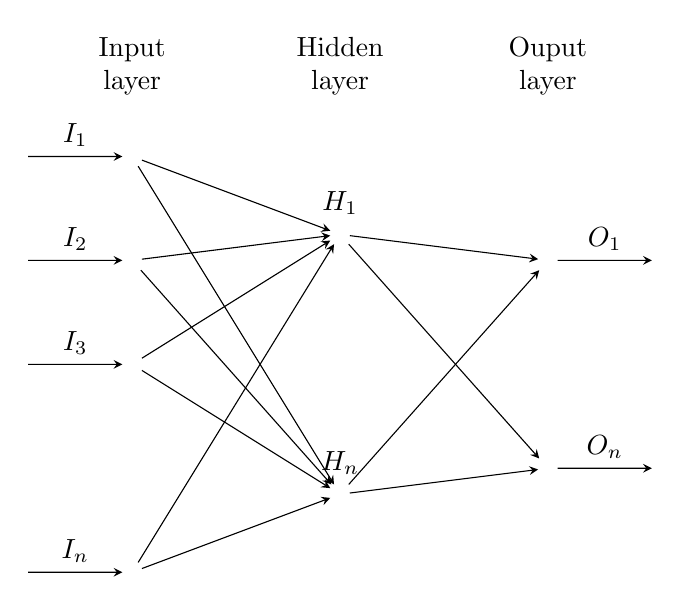
\begin{tikzpicture}[xscale=0.88, yscale=0.88,x=1.5cm, y=1.5cm, >=stealth]

\foreach \m/\l [count=\y] in {1,2,3,missing,4}
  \node [every neuron/.try, neuron \m/.try] (input-\m) at (0,2.5-\y) {};

\foreach \m [count=\y] in {1,missing,2}
  \node [every neuron/.try, neuron \m/.try ] (hidden-\m) at (2,2-\y*1.25) {};

\foreach \m [count=\y] in {1,missing,2}
  \node [every neuron/.try, neuron \m/.try ] (output-\m) at (4,1.5-\y) {};

\foreach \l [count=\i] in {1,2,3,n}
  \draw [<-] (input-\i) -- ++(-1,0)
    node [above, midway] {$I_\l$};

\foreach \l [count=\i] in {1,n}
  \node [above] at (hidden-\i.north) {$H_\l$};

\foreach \l [count=\i] in {1,n}
  \draw [->] (output-\i) -- ++(1,0)
    node [above, midway] {$O_\l$};

\foreach \i in {1,...,4}
  \foreach \j in {1,...,2}
    \draw [->] (input-\i) -- (hidden-\j);

\foreach \i in {1,...,2}
  \foreach \j in {1,...,2}
    \draw [->] (hidden-\i) -- (output-\j);

\foreach \l [count=\x from 0] in {Input, Hidden, Ouput}
  \node [align=center, above] at (\x*2,2) {\l \\ layer};

\end{tikzpicture}
\caption{Deep Networks}
\end{figure}

\section{模型、假设以及标准}
\subsection{模型}
我们将一定的比例(1:2)有变点的时间序列与无变点的时间序列的变点处的小波系数混合在一起作为训练集,每个时间序列有32个小波系数。,网络结构则为$32\longrightarrow32\longrightarrow32\longrightarrow10\longrightarrow2$的全连接网络,激活函数都为sigmoid函数。训练使用的是Adam梯度,$learning rate=0.00004$。
\subsection{数据上的预先假设}
我们由于采用了简单的全连接结构,故暂不考虑高阶高维时间序列分析,我们选取了传统方法的研究核心,即均值变点检测和方差变点检测,采用固定的跳跃值来生成数据(相对于白噪声方差),同时我们也生成了AR(1)模型中系数改变的情况的数据。(Figure 3)
\begin{figure}
\centering
\includegraphics[width=1\textwidth]{cp.jpg}
\caption{三类变点,均值,方差,AR(1)参数}
\end{figure}

\subsection{标准}
训练集一共有2000个有断点数据和4000个无断点数据,测试集则采用了100个有断点数据和100个无断点数据。神经网络使用的框架是pytorch,小波分析则使用R语言实现,具体代码详见\url{https://github.com/alex-guo-leciel/cpd-wv-dl}
\section{实验结果}
在各种不同设定的数据下,经过训练,神经网络在测试集上对是否存在变点的判断正确率均超过95\%,且神经网络收敛良好(Figure 4)

\begin{figure}
\centering
\includegraphics[width=1\textwidth]{loss.jpg}
\caption{在神经网络上定义的损失函数,其值越小代表训练效果越好}
\end{figure}

\section{总结、展望}
通过本文中的实验我们可以发现神经网络对变点检测有着极大的潜能,其强大的非线性代表能力意味着能提取到一般模型难以提取到的特征,从而可以检测到传统方法难以检测到的变点特征。在这里我们只使用了最简单的全连接网,有理由相信通过几十层的深度网络我们能够训练出检测高阶模型参数改变的网络模型,而且我们只使用了二分类网络,通过拓展,可以轻易实现多类型变点检测,我们相信神经网络在多任务高纬度高复杂度的情形下将会有更好的表现。
\subsection{工作分配}
\noindent 郭森辉:神经网络研究,编写神经网络代码,并进行调参训练\\
郑哲诗:小波分析的研究,数据生成、管理,跳跃值等参数与训练效果关系的研究\\
李玉桥:小波分析的研究,数据可视化,调参训练,撰写报告初稿
\end{document}
